% vim:ft=tex:
%
\documentclass[tikz,convert={outfile=fonctions.png}]{standalone}

    \usepackage[utf8]{inputenc}

\begin{document}
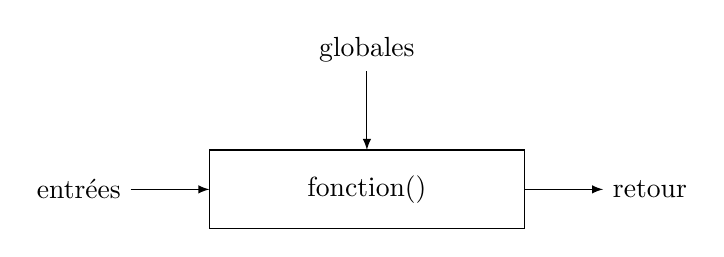
\begin{tikzpicture}[>=latex]
    \draw (0,0) rectangle (4,1) node[pos=.5] {fonction()};
    
    \draw[->] (-1,.5) node[left] {entrées} -- (0,.5);
    \draw[->] (2,2) node[above] {globales} -- (2,1);
    \draw[->] (4,.5) -- (5,.5) node[right] {retour};
\end{tikzpicture}
\end{document}

